
%(BEGIN_QUESTION)
% Copyright 2006, Tony R. Kuphaldt, released under the Creative Commons Attribution License (v 1.0)
% This means you may do almost anything with this work of mine, so long as you give me proper credit

Many types of chemical analysis are based on the sensitive detection of light.  One of the most sensitive devices available for converting a light signal into an electrical signal is a special type of electron tube known as a {\it photomultiplier tube}.  The principle of operation for this device is something called the {\it photoelectric effect}, whereby electrons may be freed from a metal surface by the collision of a photon (a ``particle'' of light):

$$\includegraphics[width=15.5cm]{i00658x01.eps}$$

A true photomultiplier tube, though, has more than just two electrodes.  There is the cathode (the most negative electrode in the tube) which emits electrons when struck by incident photons.  The anode is the most positive electrode in the tube, collecting electrons released into the vacuum.  Then, between the cathode and anode, are several other electrodes called {\it dynodes}, each one at a progressively more positive potential than the last:

$$\includegraphics[width=15.5cm]{i00658x02.eps}$$

Identify the electrodes in the above illustration, and then describe the purpose of having all those dynodes.

\vskip 20pt \vbox{\hrule \hbox{\strut \vrule{} {\bf Suggestions for Socratic discussion} \vrule} \hrule}

\begin{itemize}
\item{} What do you suppose would happen to the {\it gain} of a photomultiplier tube if the DC power supply voltage were to decrease?  Explain your reasoning.
\item{} What do you suppose would happen to the photomultiplier tube's performance if one of the voltage divider resistors were to fail open?  Explain your reasoning.
\end{itemize}

\underbar{file i00658}
%(END_QUESTION)





%(BEGIN_ANSWER)

The dynodes exhibit an effect called {\it secondary emission}, which ``multiplies'' the number of emitted electrons from the cathode.  The more dynodes, the more multiplication, which may range upward of 10$^{8}$.

%(END_ANSWER)





%(BEGIN_NOTES)

$$\includegraphics[width=15.5cm]{i00658x03.eps}$$

\vskip 20pt \vbox{\hrule \hbox{\strut \vrule{} {\bf Virtual Troubleshooting} \vrule} \hrule}

This question is a good candidate for a ``Virtual Troubleshooting'' exercise.  Presenting the diagram to students, you first imagine in your own mind a particular fault in the system.  Then, you present one or more symptoms of that fault (something noticeable by an operator or other user of the system).  Students then propose various diagnostic tests to perform on this system to identify the nature and location of the fault, as though they were technicians trying to troubleshoot the problem.  Your job is to tell them what the result(s) would be for each of the proposed diagnostic tests, documenting those results where all the students can see.

During and after the exercise, it is good to ask students follow-up questions such as:

\begin{itemize}
\item{} What does the result of the last diagnostic test tell you about the fault?
\item{} Suppose the results of the last diagnostic test were different.  What then would that result tell you about the fault?
\item{} Is the last diagnostic test the best one we could do?
\item{} What would be the ideal order of tests, to diagnose the problem in as few steps as possible?
\end{itemize}

%INDEX% Electronics review: photomultiplier tube

%(END_NOTES)


